\begin{student}
To \emph{add} is to \emph{sum}. The meanings are identical.

It is useful to think about the number line for your basic operations:

\begin{figure}[ht]
    \centering
    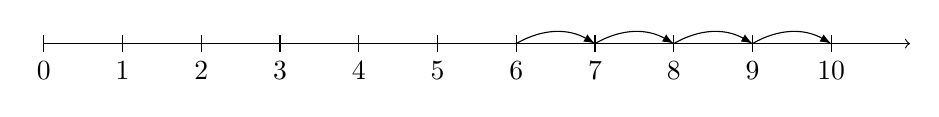
\begin{tikzpicture}
        \draw[->] (0,0) -- (11,0);
        \foreach \x in {0,1,2,3,4,5,6,7,8,9,10}
            \draw[shift={(\x,0)}] (0,3pt) -- (0,-3pt) node[below] {$\x$};
        \foreach \x in {1,2,3,4}
            \draw[-latex] (6+\x-1,0) to[bend left] (6+\x,0);
    \end{tikzpicture}
    \caption{the addition, 6 + 4}
\end{figure}

It seems trivial now, but learning to think in simple terms will help your mathematical problem solving skills\footnote{i.e. what does it mean to multiply 6 by -2 on the number line?}.
\end{student}

\subsection{Commutativity}
The algebraic operation of \emph{addition} is said to \textbf{commutative}. This means that $a + b$ is the same as $b + a$.

\begin{questions}
    \Question[1] A good way to remember this is:
    \begin{solutionordottedlines}[1in]
        If it is possible to commuting from place A to place B, then it will be the exact same commuting from place B back to place A!
    \end{solutionordottedlines}
\end{questions}

\subsection{Associativity}
Addition is also \textbf{associative}. This means that $(a + b) + c$ is the same as $a + (b + c)$. This becomes helpful in that we can just swap the order around for addition. See if you can discover this yourself:

\begin{examples}
    \begin{questions}
        \Question[2] Calculate the following. Ask your tutor for a hint if it's taking longer than 20 seconds.
        \begin{parts}
            \part $23+41+7+9 = $ \fillin[80] 
            \part $27+55+445+23+7$ \fillin[557]
        \end{parts}
    \end{questions}
\end{examples}

\begin{exercises}
    It should not take you more than 15 minutes to complete all of the following:
    \begin{questions}
        \Question[6] Half marks each; carry out the additions mentally.
        \begin{multicols}{3}
            \begin{parts}
                \part $15 + 5=$ \fillin[][1.5cm]
                \part $8+22=$ \fillin[][1.5cm]
                \part $13+7=$ \fillin[][1.5cm]
                \part $74+6=$ \fillin[][1.5cm]
                \part $7+58=$ \fillin[][1.5cm]
                \part $6+38=$ \fillin[][1.5cm]
                \part $8+89=$ \fillin[][1.5cm]
                \part $32+9=$ \fillin[][1.5cm]
                \part $35+27=$ \fillin[][1cm]
                \part $42+19=$ \fillin[][1cm]
                \part $29+36=$ \fillin[][1cm]
                \part $57+86=$ \fillin[][1cm]
            \end{parts}
        \end{multicols}
        \Question[4] Also half marks:
        \begin{multicols}{2}
            \begin{parts}
                \part \(1+9+33=\) \fillin[]
                \part \(2+38+5=\) \fillin[]
                \part \(27+6+3=\) \fillin[]
                \part \(16+24+5=\) \fillin[]
                \part \(61+9+24=\) \fillin[]
                \part \(4+42+38=\) \fillin[]
                \part \(16+55+27=\) \fillin[]
                \part \(72+19+26=\) \fillin[]
            \end{parts}
        \end{multicols}
        \Question[4] Now with 4 terms.
        \begin{multicols}{2}
            \begin{parts}
                \part \(22+17+18+23\) =\fillin[][1.5cm]
                \part \(14+18+76+92\) =\fillin[][1.5cm]
                \part \(13+27+64+6\) =\fillin[][1.5cm]
                \part \(25+32+15+18\) =\fillin[][1.5cm]
                \part \(15+34+26+35\) =\fillin[][1.5cm]
                \part \(12+19+18+1\) =\fillin[][1.5cm]
            \end{parts}
        \end{multicols}
        \Question[8] Now entering the triple digits. I'll pay you 1 mark each:
        \begin{multicols}{2}
            \begin{parts}
                \part \(243+57=\) \fillin[]
                \part \(567+43=\) \fillin[]
                \part \(328+22=\) \fillin[]
                \part \(786+24=\) \fillin[]
                \part \(435+25=\) \fillin[]
                \part \(963+57=\) \fillin[]
                \part \(486+524=\) \fillin[]
                \part \(364+251=\) \fillin[]
            \end{parts}
        \end{multicols}
        \Question[2] Three cows produced 29 litres, 47 litres and 23 litres of milk in one day. How much milk did they produce in total?
        \begin{solutionordottedlines}[1in]
        \end{solutionordottedlines}
        \Question[2] A tiler laid 267 tiles in the kitchen, 20 tiles in the laundry and 113 tiles in the bathroom. How many tiles did he lay in total?
        \begin{solutionordottedlines}[1in]
        \end{solutionordottedlines}
        \Question[2] On the first day of my holidays, I travelled 85 kilometres from my home in Victor Harbor to Adelaide, then 516 kilometres from Adelaide to Broken Hill. The next day I travelled 298 kilometres from Broken Hill to Mildura.
How many kilometres did I travel in the first two days of my trip?
        \begin{solutionordottedlines}[2in]
        \end{solutionordottedlines}
        \Question[2] A busker collected \(\$ 8.00, \$ 13.00, \$ 4.00\) and \(\$ 12.00\) over four days. How much did she earn?
        \begin{solutionordottedlines}[2in]
        \end{solutionordottedlines}
        \Question[2] In three Year 7 classes, 27 students, 31 students and 26 students attended roll call one morning. How many Year 7 students were present?
        \begin{solutionordottedlines}[2in]
        \end{solutionordottedlines}
        \Question[2] I picked 18 daffodils from my garden on Monday, 3 on Tuesday, 27 on Wednesday, 6 on Thursday and 12 on Friday. How many daffodils did I pick over the five days?
        \begin{solutionordottedlines}[2in]
        \end{solutionordottedlines}
        \Question[2] In one week, Sam read four books. The first book had 312 pages, the second 175, the third 48 and the fourth 98 . How many pages did Sam read in the week?
        \begin{solutionordottedlines}[2in]
        \end{solutionordottedlines}
        \Question[2]$\,$
        \begin{parts}
            \part By appropriately pairing numbers, carry out the addition \(1+2+3+4+5+6+7+8+9\)
            \begin{solutionordottedlines}[2in]
            \end{solutionordottedlines}
            \part Use the same idea to find the sum of numbers from 1 to 99 inclusive.
            \begin{solutionordottedlines}[2in]
            \end{solutionordottedlines}
        \end{parts}
    \end{questions}
\end{exercises}


